\documentclass[../main.tex]{subfiles}
	% COMMUNICATIONS TESTING
\begin{document}

In order to determine the noise characteristics and error rate of each communication scheme on the test bed, data is transmitted through the system and analysed with respect to the input.
For On-Off Keying, a random bit stream is generated once and then used for all of the tests so it can be compared consistently.
Not many of these tests are included, because above about \SI{500}{\hertz} Python starts to miss clock edges with the speed of the transitions, and it becomes a deletion channel instead of an error channel.
For the advanced modulation schemes, 4-Pulse Amplitude Modulation and 16-Quadrature Amplitude Modulation are tested at baseband frequencies.
The data used for these tests is a black and white image of a kitten with enough gradient and contrast to be interesting informationally, because random bit sequences are less interesting to transmit and do not provide an intuitive understanding of the noise introduced or whether the data has transmitted correctly.
The image is read into the transmitter, converted into bitmasks for the DAC, sent to the receiver, read in as bitmasks by the ADC and converted back into an image.
The transmissions are referred to in terms of baud rate or symbol rate.
This is also equivalent to the bitmask transmission rate, and is half the bit rate for 4PAM (2 bits per symbol/bitmask) and a quarter of the bit rate for 16QAM (4 bits per symbol/bitmask).\\

\begin{figure}[ht]
	\centering
	
	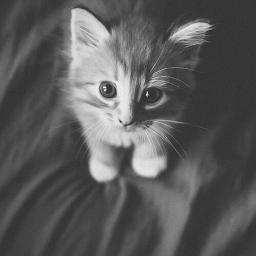
\includegraphics[width=0.26\textwidth]{cat2_bw.jpg}
	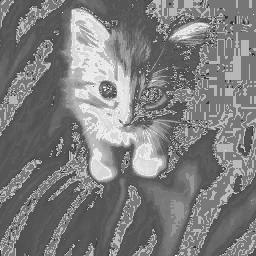
\includegraphics[width=0.26\textwidth]{cat2_out_1_4PAM_500.jpg}
	
	\caption{The original cat image (left) and the image transmitted at a baud rate of 500Hz (right)}
	\label{fig_Original Cat}
\end{figure}

Figure \ref{fig_Original Cat} shows the original cat image and the image transmitted at a low baud rate (\SI{500}{\hertz}).
Transmission was attempted for a number of slightly different lookup tables for the DAC symbols all at one frequency (including no lookup table - this produced the worst results), and this seemed to make a significant difference to the quality of the transmission -- this is a large source of error in the system.
The darkest areas of the image suffer the most from the transmission, and this could be due to the scaling of values being inclusive of noise, but it could also be due to more likely errors introduced by the components.
There was a concern that at high frequencies the transmission would start to act as a deletion channel as it did with the OOK transmission, and miss some bitmasks.
This was not a problem, however, as even at the highest frequency the ADC could handle (\SI{100}{\kilo\hertz}), the number of bitmasks received was the number expected.
Figure \ref{fig_4PAM Cats} shows the result of 4PAM transmission at different increasing baud rates from \SIrange{1}{100}{\kilo\hertz}.
The \SI{1000}{\hertz} image shows addition of salt and pepper noise relative to the \SI{500}{\hertz} image, and then Gaussian noise seems to slowly fade out the image leaving only the basic structure intact.
Interference is likely introduced by the connective wires from the GPIO to the components, which are capacitively coupled at high frequency and would explain the averaging out of the colours as frequency increases.
The final \SI{100}{\kilo\hertz} image looks like it is almost entirely random noise.

\begin{figure}[ht]
	\centering
	
	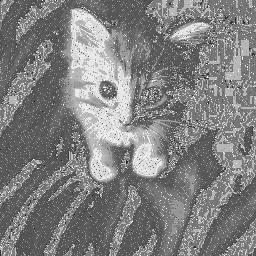
\includegraphics[width=0.26\textwidth]{cat2_out_2_4PAM_1k.jpg}
	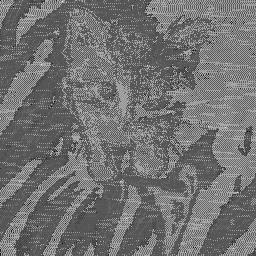
\includegraphics[width=0.26\textwidth]{cat2_out_3_4PAM_2k.jpg}
	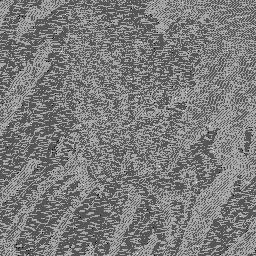
\includegraphics[width=0.26\textwidth]{cat2_out_4_4PAM_5k.jpg}\\[1mm]
	
\includegraphics[width=0.26\textwidth]{cat2_out_5_4PAM_10k.jpg}
	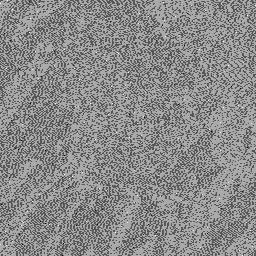
\includegraphics[width=0.26\textwidth]{cat2_out_6_4PAM_50k.jpg}
	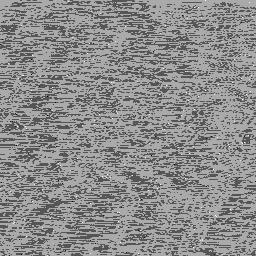
\includegraphics[width=0.26\textwidth]{cat2_out_7_4PAM_100k.jpg}
	
	\caption{Rates of transmission for 4PAM: (top) 1kHz, 2KHz, 5kHz, (bottom) 10kHz, 50kHz, 100kHz}
	\label{fig_4PAM Cats}
\end{figure}

The images for the same baud rates as Figure \ref{fig_4PAM Cats} are shown in Figure \ref{fig_16QAM Cats} for 16 QAM transmission.
These images, although different in quality, show roughly the same structural characteristics, particularly the difference between the \SI{2}{\kilo\hertz} image and the \SI{5}{\kilo\hertz} image in each, and the transition to random noise in the \SI{100}{\kilo\hertz} image in each.
The symbol rates for corresponding 4PAM and 16QAM being the same means that the bit rate for 16QAM is twice as high, although as the I and Q components of each symbol are transmitted in parallel the symbol rate is more relevant for comparison, seen in the similarities in same-baud-rate images for both sets.
The 16QAM images appear lower in quality than the 4PAM images.
There are two expected reasons for this: firstly, there are more exposed cables which can become capacitively coupled in this setup, compounding the problem, and secondly, although both DACs displayed very similar output values, the lookup table used is based on the first DAC and may not be as accurate in expressing the correct levels for the second.
Grey coding implemented in this transmission scheme should have helped to reduce the bit error rate.

\begin{figure}[ht]
	\centering
	
	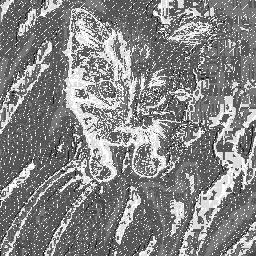
\includegraphics[width=0.26\textwidth]{cat2_out_9_16QAM_1k.jpg}
	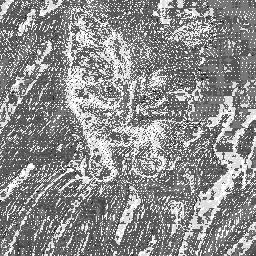
\includegraphics[width=0.26\textwidth]{cat2_out_10_16QAM_2k.jpg}
	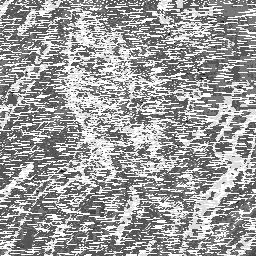
\includegraphics[width=0.26\textwidth]{cat2_out_11_16QAM_5k.jpg}\\[1mm]
	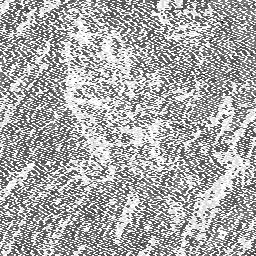
\includegraphics[width=0.26\textwidth]{cat2_out_12_16QAM_10k.jpg}
	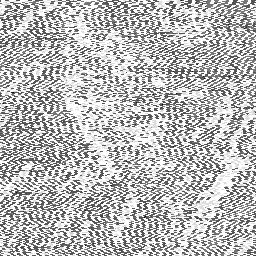
\includegraphics[width=0.26\textwidth]{cat2_out_13_16QAM_50k.jpg}
	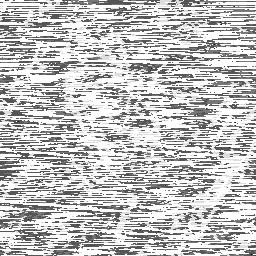
\includegraphics[width=0.26\textwidth]{cat2_out_14_16QAM_100k.jpg}
	
	\caption{Rates of transmission for 16QAM: (top) 1kHz, 2KHz, 5kHz, (bottom) 10kHz, 50kHz, 100kHz}
	\label{fig_16QAM Cats}
\end{figure}

%%%%%%%%%%%%%%%%%%%%%%%%%%%%%%%%%%%%%%%%%%%%%%%%%%%%%%%%%%%%%%%%%%%%%%%%%%%%%%%%%%%%%%%%%%%%%%%%%%%%%%%%%%%%%%%%%%%%%%%%%%%%%%%%%%

\section{Bit Error Rate}

The Bit Error Rate (BER) is simply the percentage of bits that are received in error with respect to the original transmission.
This is computed for the image transmissions of the advanced modulation schemes, and for the only test of a random bit stream transmission which yielded a same-size output for On-Off Keying, in Table \ref{tab_BER}.
The 4PAM and 16QAM results have a surprisingly high Bit Error Rate, seeming to suggest that the test bed did not perform particularly well despite visible success at lower frequencies.
However they can be seen to approach a random $50\% BER$ as the frequency increases which agrees with a visual interpretation of the data.

\begin{table}[h]
	\centering
	\global\tabulinesep = 2mm
	\begin{tabu} to 0.8\textwidth { | X[c] | X[c] | X[c] | X[c] | }
		\hline
		Baud Rate ($kHz$) & OOK BER ($\%$) & 4PAM  BER ($\%$) & 16QAM BER ($\%$)\\
		\hline\hline
		1 & 5.06 & 46.20 & 45.92\\
		\hline
		2  & -- & 45.59 & 46.31\\
		\hline
		5  & -- & 48.83 & 46.44\\
		\hline
		10 & -- & 48.96 & 46.65\\
		\hline
		50 & -- & 50.59 & 46.88\\
		\hline
		100 & -- & 50.89 & 46.80\\
		\hline
	\end{tabu}
	\caption{Table of Bit Error Rate for transmission of OOK, 4PAM and 16QAM at different baud rates}
	\label{tab_BER}
\end{table}

%%%%%%%%%%%%%%%%%%%%%%%%%%%%%%%%%%%%%%%%%%%%%%%%%%%%%%%%%%%%%%%%%%%%%%%%%%%%%%%%%%%%%%%%%%%%%%%%%%%%%%%%%%%%%%%%%%%%%%%%%%%%%%%%%%

\section{Signal to Noise Ratio}

The Signal to Noise Ratio (SNR) is calculated as the ratio of the signal power to the noise power in the system, where power is the mean squared value of the amplitude of the signal.
\begin{equation}
	SNR = \frac{P_{signal}}{P_{noise}} = \left(\frac{A_{signal (RMS)}}{A_{noise (RMS)}}\right)^2
\end{equation}

The Root-Mean-Squared (RMS) amplitude of the signal is calculated from the symbols which were transmitted.
The amplitude of the noise is taken as the difference between the received values stored in the receiver's bitmasks (before Maximum Likelihood estimation is performed), and the symbols they represent.
A graph of SNR against frequency is produced in Figure \ref{fig_4PAM SNR} for 4PAM and 16QAM.
The SNR of the test bed as measured is not particularly large, with a large noise component.
The SNR can also be seen to drop off at higher frequencies, which is expected from the unshielded wire setup, and this is clear in the images.
The 4PAM SNR plot (red) is expected to be higher due to fewer wires with which to interfere, it would therefore be expected to drop off less quickly as the frequency increased, although whether the plot is characteristic of the system is unclear	.\\

\begin{figure}[ht]
	\centering
	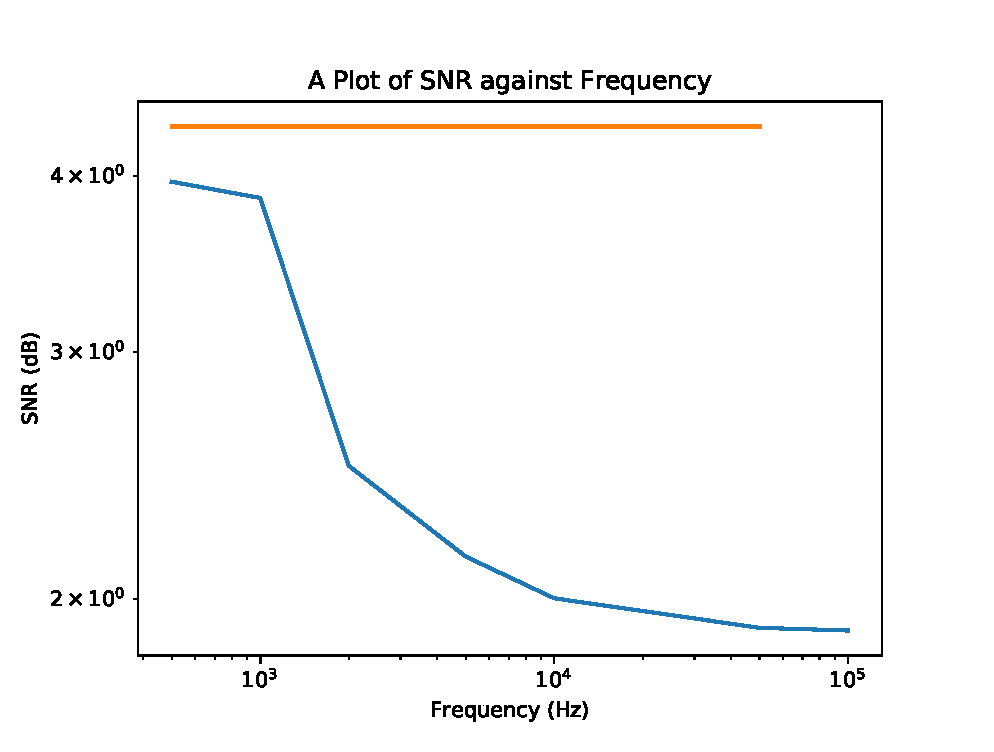
\includegraphics[width=0.6\textwidth]{SNR_Plot.eps}	
	\caption{Figure of SNR against Frequency for 4PAM (red) and 16QAM (yellow)}
	\label{fig_4PAM SNR}
\end{figure}


%%%%%%%%%%%%%%%%%%%%%%%%%%%%%%%%%%%%%%%%%%%%%%%%%%%%%%%%%%%%%%%%%%%%%%%%%%%%%%%%%%%%%%%%%%%%%%%%%%%%%%%%%%%%%%%%%%%%%%%%%%%%%%%%%%

\section{Channel Coding} \label{sec_Channel Coding}

Channel coding was intended to be included as Hamming Codes, implementing forward error correction through syndrome decoding.
Unfortunately due to time constraints and component issues, this was not included.
However, there is a very interesting Python library which would allow for easy integration of more complex error correction, \textit{CommPy} \cite{lib_CommPy}.
It includes convolutional codes with Viterbi and MAP decoders, Turbo Code encoding and decoding and random interlevers and de-interlevers.

\end{document}